\chapter{Diseño de datos}
En este apartado se obtendrá el modelo relacional a partir de los diagramas de la base de datos del apartado \ref{analisis-tipos-entidad}. El modelo relacional se compone de los elementos que se indican a continuación:

\subsubsection*{Entidad}
Cada una de las tablas que componen el modelo.

\subsubsection*{Atributo} Es una columna de una tabla. Cada una tiene un nombre y un dominio asociados.

\subsubsection*{Dominio}
Es el conjunto de valores que puede tomar un campo.

\subsubsection*{Tupla}
Es un conjunto formado por un valor de cada atributo de la tabla. No pueden existir dos tuplas iguales en una tabla.

\subsubsection*{Clave}
Es el atributo o conjunto de atributos de una tabla por cuyos valores identifica unívocamente a cada tupla.

Para generar el modelo relacional a partir del esquema entidad-interelación se utilizan las reglas de normalización y transformación que se indican en \textit{Bases de datos: desde Chen hasta Codd con Oracle} \cite{basesdedatos-rama} que evitan redundancias y problemas de integridad en los datos. En este caso se han tomado algunas decisiones de diseño que facilitarán más adelante la implementación y que se indican a continuación:

\begin{enumerate}
    \item Se utilizan claves autonuméricas para todas las tablas.
\end{enumerate}


En la figura \ref{fig:esquema-relacional} se representan todas las tablas, relaciones, atributos y claves del esquema relacional de la base de datos de \emph{PushNews}.

\begin{figure}[ht]
    \centering
    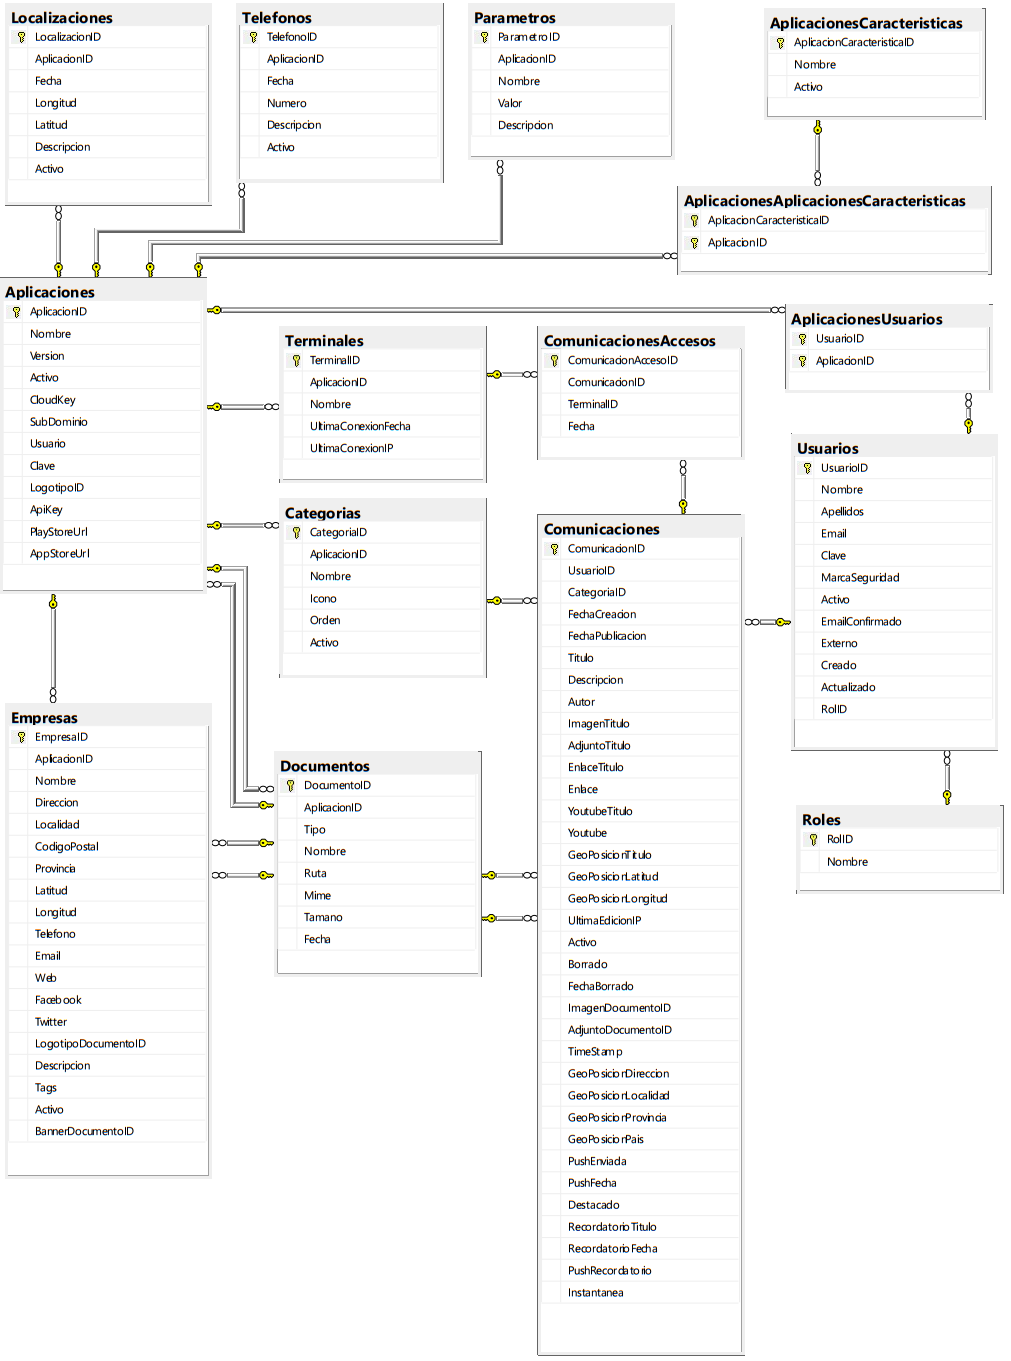
\includegraphics[scale=.59]{esquema_base_datos}
    \caption{Esquema relacional}
    \label{fig:esquema-relacional}
\end{figure}
